\documentclass[11pt]{article}
\usepackage[utf8]{inputenc}
\usepackage{amsmath,amssymb,amsthm}
\usepackage{graphicx}
\usepackage{hyperref}
\usepackage{algorithm}
\usepackage{algorithmic}
\usepackage{booktabs}
\usepackage{wrapfig}

\title{ *WIP* tatbot: Tattoo Robot}
\author{Hugo Ponte}
\date{\today}

\begin{document}
\maketitle

\begin{figure}[h]
    \centering
    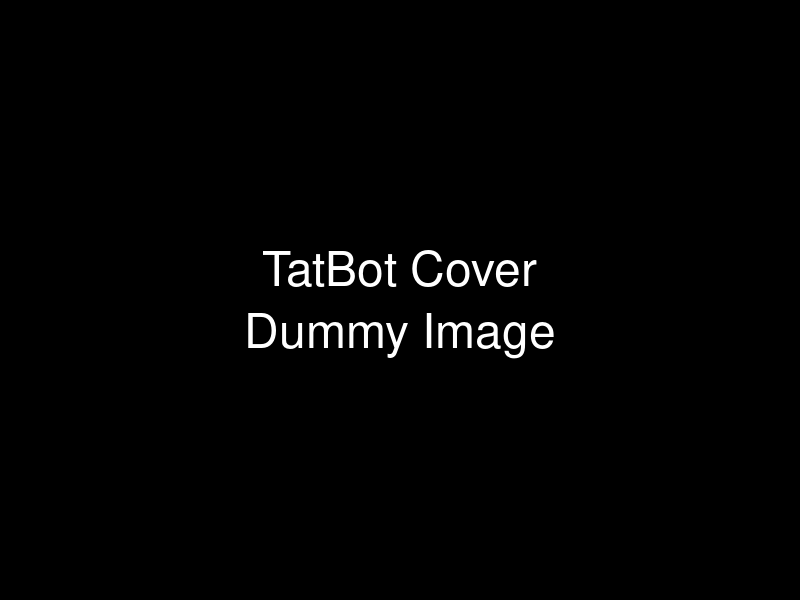
\includegraphics[width=0.8\textwidth]{figures/cover.png}
    \caption{(a) The tatbot system (hardware v0.2) (b) First human tattoo performed by the tatbot system. }
    \label{fig:cover}
\end{figure}


\begin{abstract}
We present \textbf{TatBot}, an autonomous robotic system that demonstrates the feasibility of AI-powered robotic tattooing through sophisticated hardware integration and advanced software architecture.
The system employs a distributed computing infrastructure with specialized nodes for perception, AI inference, and robot control, enabling real-time tattoo generation and execution.
TatBot features dual Trossen Robotics WidowXAI arms with precision tattoo machines, Intel RealSense depth cameras for 3D perception, and a comprehensive software stack leveraging JAX for GPU-accelerated inverse kinematics and geodesic surface mapping.
The system has achieved significant milestones including the first successful robotic tattoo on May 20, 2025, and has evolved through four hardware iterations and five software versions.
Key technical innovations include a unified MCP server architecture for distributed control, sophisticated 3D surface mapping using potpourri3d for geodesic path tracing, and an advanced IK solver employing JAX Least Squares optimization with trust region methods.
The artwork generation pipeline integrates DrawingBotV3 for vectorization and Replicate Playground for AI-powered design creation, demonstrating the potential for autonomous artistic expression in body modification.
TatBot represents a new paradigm in robotic artistry, bridging the gap between human creativity and machine precision in the ancient art of tattooing, while maintaining the cultural and personal significance of body art through AI-powered robotics.
\end{abstract}

\pagebreak

\begin{figure}[h]
    \centering
    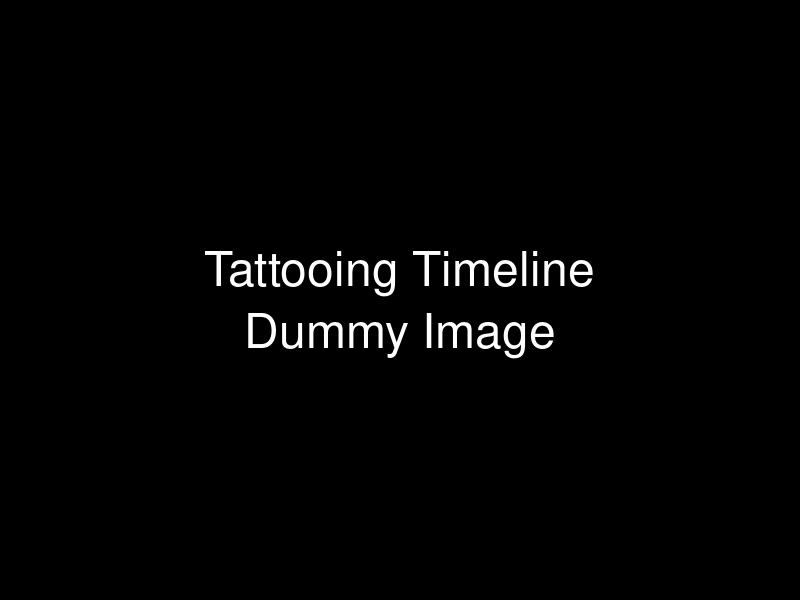
\includegraphics[width=0.8\textwidth]{figures/timeline.png}
    \caption{A history of tattoos.}
    \label{fig:timeline}
\end{figure}

\section{Background}

\subsection{History}

Tattoos are an ancient art form that predates recorded history.
Tattoos have been used as punishment, status symbols, and even therapeutic tools.
Ötzi, a frozen mummy found in the alps dated to 6272 BP, had tattoos on his arthritic joints \cite{deterwolf_worlds_oldest}.
The Yimkhiungs of Northern India perform ritualized tattooing on children as young as 5 yearls old \cite{kluger2015cultural}.
In ancient Mesopotamia, tattooing was used to mark slaves to punitively identify criminals \cite{hawken2022tattooing}.
Today tattoos have evolved and merged into a global art form that is practiced in every corner of the world.
Though some of the original symbology and purpose still remains, most modern tattoos are purely aesthetic.
In many cultures, tattoos have to be "earned". They might represent a rite of passage, family sigil, or national identy. There is still debate over cultural appropriation of tattoos.
Tattoo comes from a polynesian word \textit{tatau} which means \textit{to strike}, a reference to the traditional method of tattooing where needle penetration is achieved by striking with stick.
During the 18th and 19th centuries, the age of exploration introduced Polynesian tattoos to the west.
As a result, most modern languages now use the loanword tattoo to describe the art form over whatever traditional terminology may have existed.
Tattooing is one of the oldest forms of body modification, with evidence dating back to the Neolithic period. The earliest known tattoos belong to "Otzi the Iceman, a 5,300-year-old mummy discovered in the "Otztal Alps, featuring 61 carbon-based tattoos likely placed for therapeutic purposes on arthritic joints \cite{Samadelli2015,deterwolf_worlds_oldest}. Similar ancient tattoos have been identified on Egyptian mummies from around 2000 BCE, including figurative designs possibly linked to fertility and protection \cite{friedman2018natural}. In the Americas, the oldest tattoos appear on a Chinchorro mummy from Chile, dated to 2563--1972 BCE, consisting of dotted lines \cite{arrietamummies}. Across prehistoric and ancient societies, tattoos served diverse functions: medicinal and protective in Europe and Egypt; markers of social status, lineage, and rites of passage in Austronesian cultures like those in Polynesia and Micronesia \cite{kluger2015cultural}; and symbols of achievement or spiritual significance among indigenous groups in North America, such as the Osage and Haudenosaunee \cite{deterwolf2013drawing}.
In various ancient civilizations, tattooing also carried punitive connotations. In Mesopotamia, it was used to brand slaves and criminals \cite{hawken2022tattooing}, a practice echoed in Greco-Roman societies where tattoos stigmatized captives, deserters, and gladiators \cite{jones1987stigma}. Among the Thracians, however, tattoos signified nobility. In Asia, Chinese and Japanese tattoos evolved from spiritual markings to punitive brands during certain periods, influencing modern Yakuza traditions \cite{krutak2012tattooing}. Indigenous practices, such as the hand-tapped tattoos of Samoa (pe'a for men, malu for women), emphasized endurance and social hierarchy, while Inuit women used facial tattoos (kakiniit) to denote maturity and spiritual readiness \cite{johnston2017reawakening}.
The term tattoo'' derives from the Polynesian word \textit{tatau}, meaning to strike,'' referring to traditional tapping methods with bone tools. European contact during the Age of Exploration, notably Captain James Cook's voyages in the 18th century, introduced Polynesian tattooing to the West, leading to its adoption among sailors and eventual integration into global terminology \cite{friedman2014cook}. By the 19th century, tattoos spread through colonial encounters, often associated with marginal groups like convicts and military personnel.
In contemporary society, tattooing has transformed into a widespread art form practiced worldwide, blending traditional symbolism with aesthetic expression. While some cultures retain ``earned'' tattoos representing rites of passage or heritage---such as those among the Yimkhiung of Northern India, where children as young as five undergo ritual tattooing \cite{kluger2015cultural}---most modern tattoos are decorative. Debates persist over cultural appropriation, particularly of indigenous designs. The Tattoo Renaissance since the 1970s has mainstreamed the practice, driven by technological advancements like the electric tattoo machine (patented in 1891) and media exposure, with tattoos now symbolizing personal identity, reclamation, and artistic innovation \cite{schildkrout2004inscribing,roberts2012secret}.

\subsection{Biology}

\begin{wrapfigure}{l}{0.5\textwidth}
    \vspace{-20pt}
    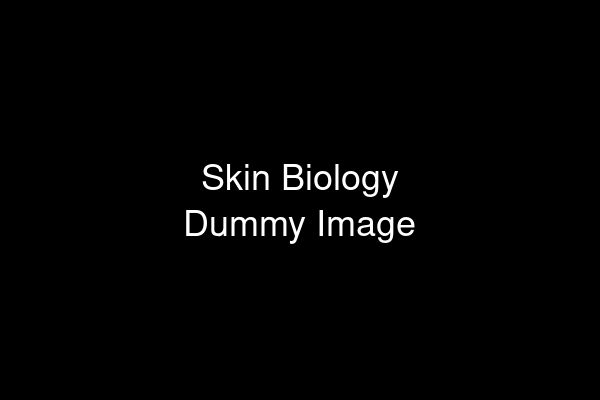
\includegraphics[width=\linewidth]{figures/biology.png}
    \caption{Skin layers and tattoo biology.}
    \label{fig:biology_wrap}
\end{wrapfigure}

The human skin is a complex organ, but it can roughly be divided into three layers:

\begin{itemize}
    \item Epidermis: outermost layer, 0.1 to 0.5mm thick, contains melanocytes, keratinocytes, and melanin.
    \item Dermis: middle layer, 1 to 4mm thick, contains blood vessels, nerves, and hair follicles.
    \item Subcutaneous tissue: innermost layer, 1 to 4mm thick, contains fat and connective tissue.
\end{itemize}

In a perfect tattoo, each needle puncture will deposit ink particles into the dermis.
Ink deposited in the epidermis will fade as the skin cells regenerate.
Ink deposited in the subcutaneous tissue will "blow out" as it diffuses outwards from the puncture site.
because tattoos penetrate the skin, they can be a vector for disease transmission.
medical grade equipment and sanitation protocols are required to prevent infection.

\begin{figure}[h]
    \centering
    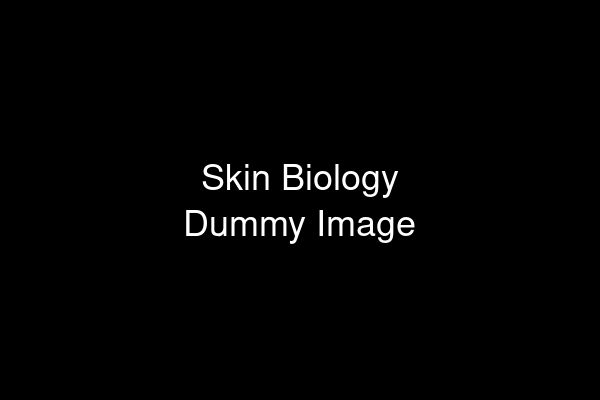
\includegraphics[width=0.8\textwidth]{figures/biology.png}
    \caption{Skin layers and tattoo biology showing epidermis, dermis, and subcutaneous tissue.}
    \label{fig:biology}
\end{figure}

\pagebreak

\subsection{Technology}

Tattoo machines can be classified into two rough categories: rotary and coil.
rotary machines have become the standard for modern tattooing.
a wide variety of manufacturers compete to create the best wireless battery powered rotary machines.
voltage is modulated to control the speed of the motor, ranging from 3V to 12V.
needles are sold in pre-packaged cartridges, providing a convenient sterilized one-time use needle.
many cartridge types and vendors exist
needles are classified by their diameter, a grouping pattern, taper type, and length.
rotary machines use the rotational motion of a small electric motor to drive the up and down motion of the needle.
The distance the needle travels is called the \textit{stroke length}.

\begin{figure}[h]
    \centering
    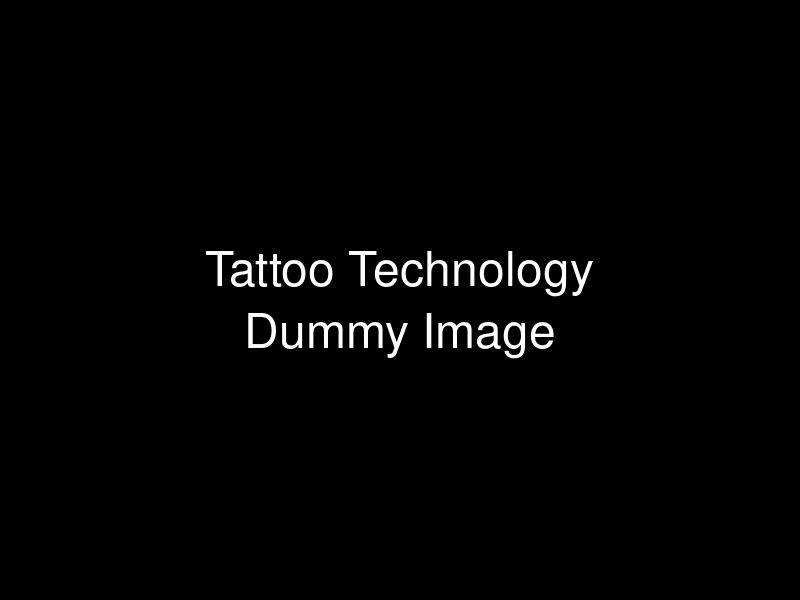
\includegraphics[width=0.8\textwidth]{figures/technology.png}
    \caption{Tattoo machine technology showing rotary and coil machine components.}
    \label{fig:technology}
\end{figure}

\subsection{Theory}

A tattoo $T = (s_1, s_2, \ldots, s_n)$ is a sequence of $n$ strokes $s_i$.
A stroke $s_i$ is sequence of needle poses $p_i$.
Each pose represents the position $\mathbf{p}_i \in \mathbb{R}^3$ and orientation quaternion $\mathbf{q}_i \in \mathbb{H}$.
The optimal angle of the needle is perpendicular to the skin surface.
We approximate this surface using a mesh $M_i$, which is a collection of vertices $V_i$, edges $E_i$, and faces $F_i$.
The arm is controlled in joint space $\mathbf{q} = (q_1, q_2, \ldots, q_j)$ where the number joints $J$ is $6$.
Inverse kinematics (IK) is the process that converts the joint space coordinates \( \mathbf{q} \) into the end effector space coordinates \( (\mathbf{p}_{ee}, \mathbf{q}_{ee}) \):
\[
\text{IK}: \mathbf{q} \mapsto (\mathbf{p}_{ee}, \mathbf{q}_{ee})
\]

The IK solver uses JAX Least Squares optimization with configurable weights for position, orientation, joint limits, and rest pose constraints.
The optimization employs a trust region solver with adaptive lambda parameters for robust convergence.
GPU-accelerated batch IK processing enables efficient computation of joint trajectories for entire stroke sequences.
Surface mapping employs geodesic tracing using the potpourri3d library to wrap 2D designs onto 3D curved surfaces.
The mapping pipeline includes Open3D mesh processing, KDTree-based closest point projection, and jaxlie SE3 transformations.
Stroke data structures support multiple coordinate systems with efficient array file management for large trajectory datasets.

\pagebreak

\section{tatbot}

\subsection{Hardware}

TatBot uses a pair of Trossen Robotics WidowXAI arms driven by dedicated controller boxes on a gigabit Ethernet network.
The system employs a distributed computing architecture with multiple specialized nodes connected through shared SSH keys for seamless communication.
The network topology consists of two 8-port gigabit switches: a main LAN switch and a PoE switch for camera connectivity.
The main LAN switch connects to the compute nodes and arm controllers, while the PoE switch powers and connects the overhead cameras.

Perception is handled by two Intel RealSense D405 cameras---one mounted on the right arm and another mounted overhead---along with five Amcrest 5MP PoE turret cameras providing overhead coverage.
The RealSense cameras provide 1280×720 RGBD data at 90fps depth sensing with USB3 connectivity.
The Amcrest IP5M-T1179EW-AI-V3 cameras operate at 1920×1080 resolution, 30fps, with 132° field of view and Power-over-Ethernet connectivity.
All cameras are calibrated using AprilTag-based extrinsic calibration to determine their precise 3D poses relative to the world origin.

The compute infrastructure includes an NVIDIA Jetson AGX Orin for AI inference, a System76 Meerkat PC for visualization and control, an Acer Nitro V 15 laptop for development, and two Raspberry Pi 5 computers for auxiliary tasks.
The Jetson AGX Orin provides 200 TOPS of AI inference capability with 12-core ARM Cortex-A78AE processors and 32GB unified RAM.
The Acer Nitro V 15 features an Intel i7-13620H 16-core processor with NVIDIA RTX 4050 graphics providing 194 TOPS for development and visualization tasks.
The System76 Meerkat PC serves as the primary control node with Intel i5-1340P 16-core processor and 15GB RAM.
Two Raspberry Pi 5 computers provide auxiliary compute with ARM Cortex-A76 4-core processors and 8GB RAM each.

The tattoo application system consists of two Ambition Lutin rotary tattoo machines with 3.8mm straight drive bar stroke cams, powered by swappable 2200mAh RCA batteries operating at 5-12V with ±0.1V precision adjustment.
The tattoo machines feature LED displays showing working voltage, working time, frequency, and remaining power.
The system uses 1005RL and EN05S-50-1003RL cartridge needles for precise ink deposition.
Nighthawk Black and Gstartoo color series inks provide the pigment for tattoo creation.
The system supports multiple fake skin types for testing: thin 3mm hard silicone (SOTICA brand, 7.48" × 5.62"), 5mm soft silicone with sponge backing (VTurboWay brand, 4.9" × 3.6" × 1.7"), and 2mm hard silicone with foam backing for arm simulation (HUOXOU brand, 24.8" × 4.72" × 3.94").

\begin{table}[h]
    \centering
    \caption{Compute and camera devices used by TatBot}
    \label{tab:hardware-devices}
    \begin{tabular}{lll}
        \toprule
        Device & Type & Specifications \\
        \midrule
        Jetson AGX Orin (\texttt{ojo}) & Compute & 12-core ARM Cortex-A78AE @ 2.2GHz, 32GB RAM, 200 TOPS \\
        Acer Nitro V 15 (\texttt{ook}) & Compute & Intel i7-13620H 16-core @ 3.6GHz, 16GB RAM, RTX 4050 6GB \\
        System76 Meerkat (\texttt{eek}) & Compute & Intel i5-1340P 16-core @ 4.6GHz, 15GB RAM \\
        Raspberry Pi~5 $\times$2 (\texttt{rpi1}, \texttt{rpi2}) & Compute & ARM Cortex-A76 4-core @ 2.4GHz, 8GB RAM each \\
        Intel RealSense D405 $\times$2 & Camera & 1280×720 RGBD, 90fps depth, USB3 connection \\
        Amcrest IP5M-T1179EW-AI-V3 $\times$5 & Camera & 5MP, 1920×1080, 5fps, 132° FOV, PoE \\
        \bottomrule
    \end{tabular}
\end{table}

\subsection{Software}

The TatBot system relies on a suite of open-source software packages organized into modular dependency groups with a distributed architecture powered by Model Context Protocol (MCP) servers.
The system uses Hydra for configuration management, allowing modular composition of different components (arms, cameras, scenes) from separate YAML files.
Pydantic provides schema validation and type safety, ensuring all configuration parameters are properly validated before system initialization.
The configuration system supports scene-specific setups, enabling rapid switching between different tattoo designs and experimental configurations.

\begin{itemize}
    \item \textbf{Core Dependencies:} The system uses \texttt{uv} for dependency management with Python 3.11.10. Core packages include \texttt{mcp} (v1.11.0) for Model Context Protocol communication, \texttt{paramiko} (v3.5.1) for SSH-based distributed computing, \texttt{pyroki} for robotics kinematics and trajectory planning, \texttt{huggingface-hub} (v0.34.3) for model and dataset management, and \texttt{hydra-core} for configuration orchestration.
    
    \item \textbf{Robot Control (\texttt{bot}):} \texttt{lerobot[tatbot,smolvla]} with TatBot-specific extensions for robot control, \texttt{trossen-arm} (v1.8.5) for WidowXAI arm interfacing, and \texttt{evdev} (v1.9.2) for input device handling.
    
    \item \textbf{Computer Vision (\texttt{cam}):} \texttt{lerobot[intelrealsense]} for RealSense integration, \texttt{pupil-apriltags} (v1.0.4.post11) for fiducial marker detection, and \texttt{pyrealsense2} (v2.55.1.6486) for Intel RealSense camera integration.
    
    \item \textbf{AI/ML Generation (\texttt{gen}):} \texttt{open3d} (>=0.18.0) for 3D data processing, \texttt{potpourri3d} (v1.3.0) for 3D geometry operations, and \texttt{jax[cuda12]} (>=0.4.0,<0.5.0) for GPU-accelerated numerical computation with \texttt{jaxtyping} (>=0.2.25,<1.0.0) for type annotations and \texttt{jaxlie} (>=1.3.4,<2.0.0) for Lie theory operations.
    
    \item \textbf{Image Processing (\texttt{img}):} \texttt{opencv-python} (v4.11.0.86) for image processing and \texttt{Pillow} (>=9.0.0,<11.0.0) for image manipulation.
    
    \item \textbf{Visualization (\texttt{viz}):} \texttt{viser} (v1.0.0) for 3D visualization and interactive browser-based GUIs, and \texttt{pyliblzfse} (>=0.4.1) for data compression.
    
    \item \textbf{Development (\texttt{dev}):} \texttt{isort} and \texttt{ruff} for code formatting and linting, with \texttt{pydantic-yaml} for YAML schema validation.
\end{itemize}

The system employs a unified MCP server architecture that runs on all nodes with dynamic tool registration and type-safe communication.
Each compute node runs a single, generic MCP server with node-specific behavior defined through Hydra configuration files.
The unified server architecture enables dynamic tool registration, with tools enabled or disabled via YAML configuration files.
The distributed architecture allows for load balancing and fault tolerance, with critical tasks distributed across multiple nodes.
Network file system (NFS) sharing enables seamless data exchange between nodes, with the Raspberry Pi 5 serving as the NFS server.
The software stack leverages modern Python packaging with \texttt{uv} for fast dependency resolution and virtual environment management.
MCP server logs are written to shared NFS storage for centralized monitoring and debugging across the distributed system.
Development tools include \texttt{ruff} for linting and formatting, \texttt{isort} for import organization, and comprehensive testing frameworks.
The system employs sophisticated data structures with JAX arrays for GPU-accelerated computation and efficient memory management.
Stroke data supports multiple coordinate systems with automatic file-based array storage for large trajectory datasets.
The artwork generation pipeline integrates DrawingBotV3 for vectorization and Replicate Playground for AI-powered design creation.

\subsection{VLA}

Vision-Language-Action (VLA) models represent a new paradigm in robotics, enabling systems to interpret visual inputs, understand natural language instructions, and generate complex action sequences in the real world.
Recent advances such as $\pi$0 \cite{Black2024pi0}, GR00T N1 \cite{Bjorck2025gr00t}, and SmolVLA \cite{Shukor2025smolvla} have demonstrated the potential of large-scale, generalist VLA models to perform a wide range of tasks across diverse robotic platforms.
These models leverage massive datasets and transformer-based architectures to bridge the gap between perception, language, and control, paving the way for more flexible and capable autonomous agents.

\subsection{Data Recipe}

The TatBot system employs a sophisticated artwork generation pipeline that transforms high-level design concepts into executable robotic trajectories.
The pipeline begins with image generation using Replicate Playground for initial design creation.
Vectorization is performed using DrawingBotV3 premium version with custom pen settings and G-code configurations.
Custom configuration files define pen parameters, G-code output formats, and design areas for different skin types.
The system supports multiple coordinate systems including meter coordinates, pixel coordinates, and end-effector poses.
Stroke data structures efficiently manage large trajectory datasets with separate array file storage for scalability.
Designs are stored in shared NFS storage with organized directory structures for easy access and version control.
The pipeline integrates with HuggingFace for model and dataset management, enabling cloud-based AI capabilities.
Real data collection from recorded TatBot sessions provides training data for machine learning models.
Synthetic data generation uses heuristic simulation to create diverse training scenarios.
The system leverages modern pretrained transformers to encode neural programs from internet-scale human data.
These neural programs serve as useful starting points for robotic control through transfer learning techniques.

\section{Results}

The TatBot system has achieved significant milestones in robotic tattooing, demonstrating the feasibility of autonomous tattoo application.
The first successful tattoo was completed on May 20, 2025, marking a breakthrough in robotic body art creation.
The system has evolved through four major hardware iterations (0.1 to 0.4) and five software versions (0.0.1 to 0.5.4), showing continuous improvement and refinement.
Hardware version 0.4 represents the current production system with optimized mechanical design and enhanced tattoo machine integration.
Software version 0.5.4 includes advanced AI-powered design generation capabilities and real-time control systems.
The system successfully integrates multiple tattoo machine types, including the Ambition Lutin rotary machines with precise voltage control.
Fake skin testing has been conducted using multiple skin types: thin 3mm hard silicone, 5mm soft silicone with sponge backing, and 2mm hard silicone with foam backing for arm simulation.
The distributed computing architecture has proven effective for real-time tattoo generation and execution across multiple specialized nodes.
Camera calibration using AprilTag-based extrinsic calibration has enabled precise 3D positioning and tracking.
The system demonstrates the potential for autonomous artistic expression through robotic control of traditional tattooing techniques.

\section{Discussion}

\subsection{Other Robotic Tattoo Systems}

Tattoos are fundamentally 3D.
They flow over the surfaces and curves of the body.
Every single previous robotic tattoo system has been constrained to the 2D plane.
Robot arms have been used before, but the control is still classical.
A set of waypoints are programmed by the human operator and the robot arm just simply executes.
Modern attempts have focused on 2D gantry systems, similar to 3D printers.
Even the designs are not AI generated, but rather come from a library of pre-existing human designs.
These robots are not artists, they are printers.
Technology has advanced and we need to create new systems that go beyond these limitations.
AI generated designs that are 3D by nature tattooed using a robotic arm controlled by AI.
Using modern imitation learning and reinforcement learning.

foo \cite{NietoBastida2023}
foo \cite{arar2025swiftsketch}
foo \cite{carlier2020deepsvg}
foo \cite{mellor2020unsupervised}
foo \cite{ha2017neural}
foo \cite{huang2019learning}
foo \cite{kotani2019teaching}

Various tattoo robots based on modified 3D printers have been demonstrated on YouTube \cite{EmilyTheEngineer2025}, a similar system \cite{YamanDeif2021}

\subsection{Robotic Artistry}

technology can create social tensions.
photography was frowned upon by those who feared it would replace portraiture.
robotic tattooing will run into tensions with human tattoo artists.
new art mediums do not replace old art mediums, they simply expand the canvas with which humanity can express itself.

\subsection{Future Work}

As it stands, tatbot is still just a proof of concept.
The design space is limited, the accuracy is still suboptimal.
My dream is to continue to work on this project, expanding it accross the world.
Cities are the heart of tattoing, where a large population creates an endless supply of skin.

\section{Conclusion}

The TatBot system represents a significant advancement in robotic body art, demonstrating the feasibility of autonomous tattoo application through sophisticated hardware and software integration.
The system has successfully evolved from a proof-of-concept to a functional robotic tattoo platform through four hardware iterations and five software versions.
Key achievements include the first successful robotic tattoo on May 20, 2025, and the development of a distributed computing architecture capable of real-time tattoo generation and execution.
The integration of traditional tattooing techniques with modern robotics and AI demonstrates the potential for autonomous artistic expression in body modification.
The system's modular design and open-source software stack provide a foundation for future development and broader adoption in the tattoo industry.
TatBot represents a new paradigm in robotic artistry, bridging the gap between human creativity and machine precision in the ancient art of tattooing.
The project demonstrates the potential for AI-powered robotics to expand human artistic capabilities while maintaining the cultural and personal significance of body art.
Future development will focus on improving accuracy, expanding design capabilities, and enabling human tattoo application in controlled environments.
The TatBot system opens new possibilities for the intersection of robotics, AI, and human artistic expression, potentially transforming the landscape of body modification technology.

\bibliographystyle{plain}
\bibliography{references}

\end{document} 